\section{Tracking multiobjeto en vídeo deportivo}

El tracking multiobjeto es una tarea especialmente compleja en fútbol debido a las oclusiones, los cruces entre jugadores, la similitud visual entre compañeros de equipo, los cambios de cámara y las detecciones intermitentes. Estas dificultades han motivado el uso de distintos enfoques de asociación temporal y reidentificación para mantener identidades consistentes a lo largo del vídeo.

Una alternativa habitual es DeepSORT, propuesto por \citet{WojkeDeepSORT2017}, que extiende SORT incorporando descriptores de apariencia aprendidos mediante redes de reidentificación. Además de la predicción de movimiento mediante el filtro de Kalman \citep{Kalman1960}, DeepSORT compara las detecciones con las trayectorias activas utilizando tanto información geométrica como apariencia visual. La \hyperref[fig:deepsort-esquema]{Figura~\ref*{fig:deepsort-esquema}} muestra un esquema general de este funcionamiento.

\begin{figure}[H]
    \centering
    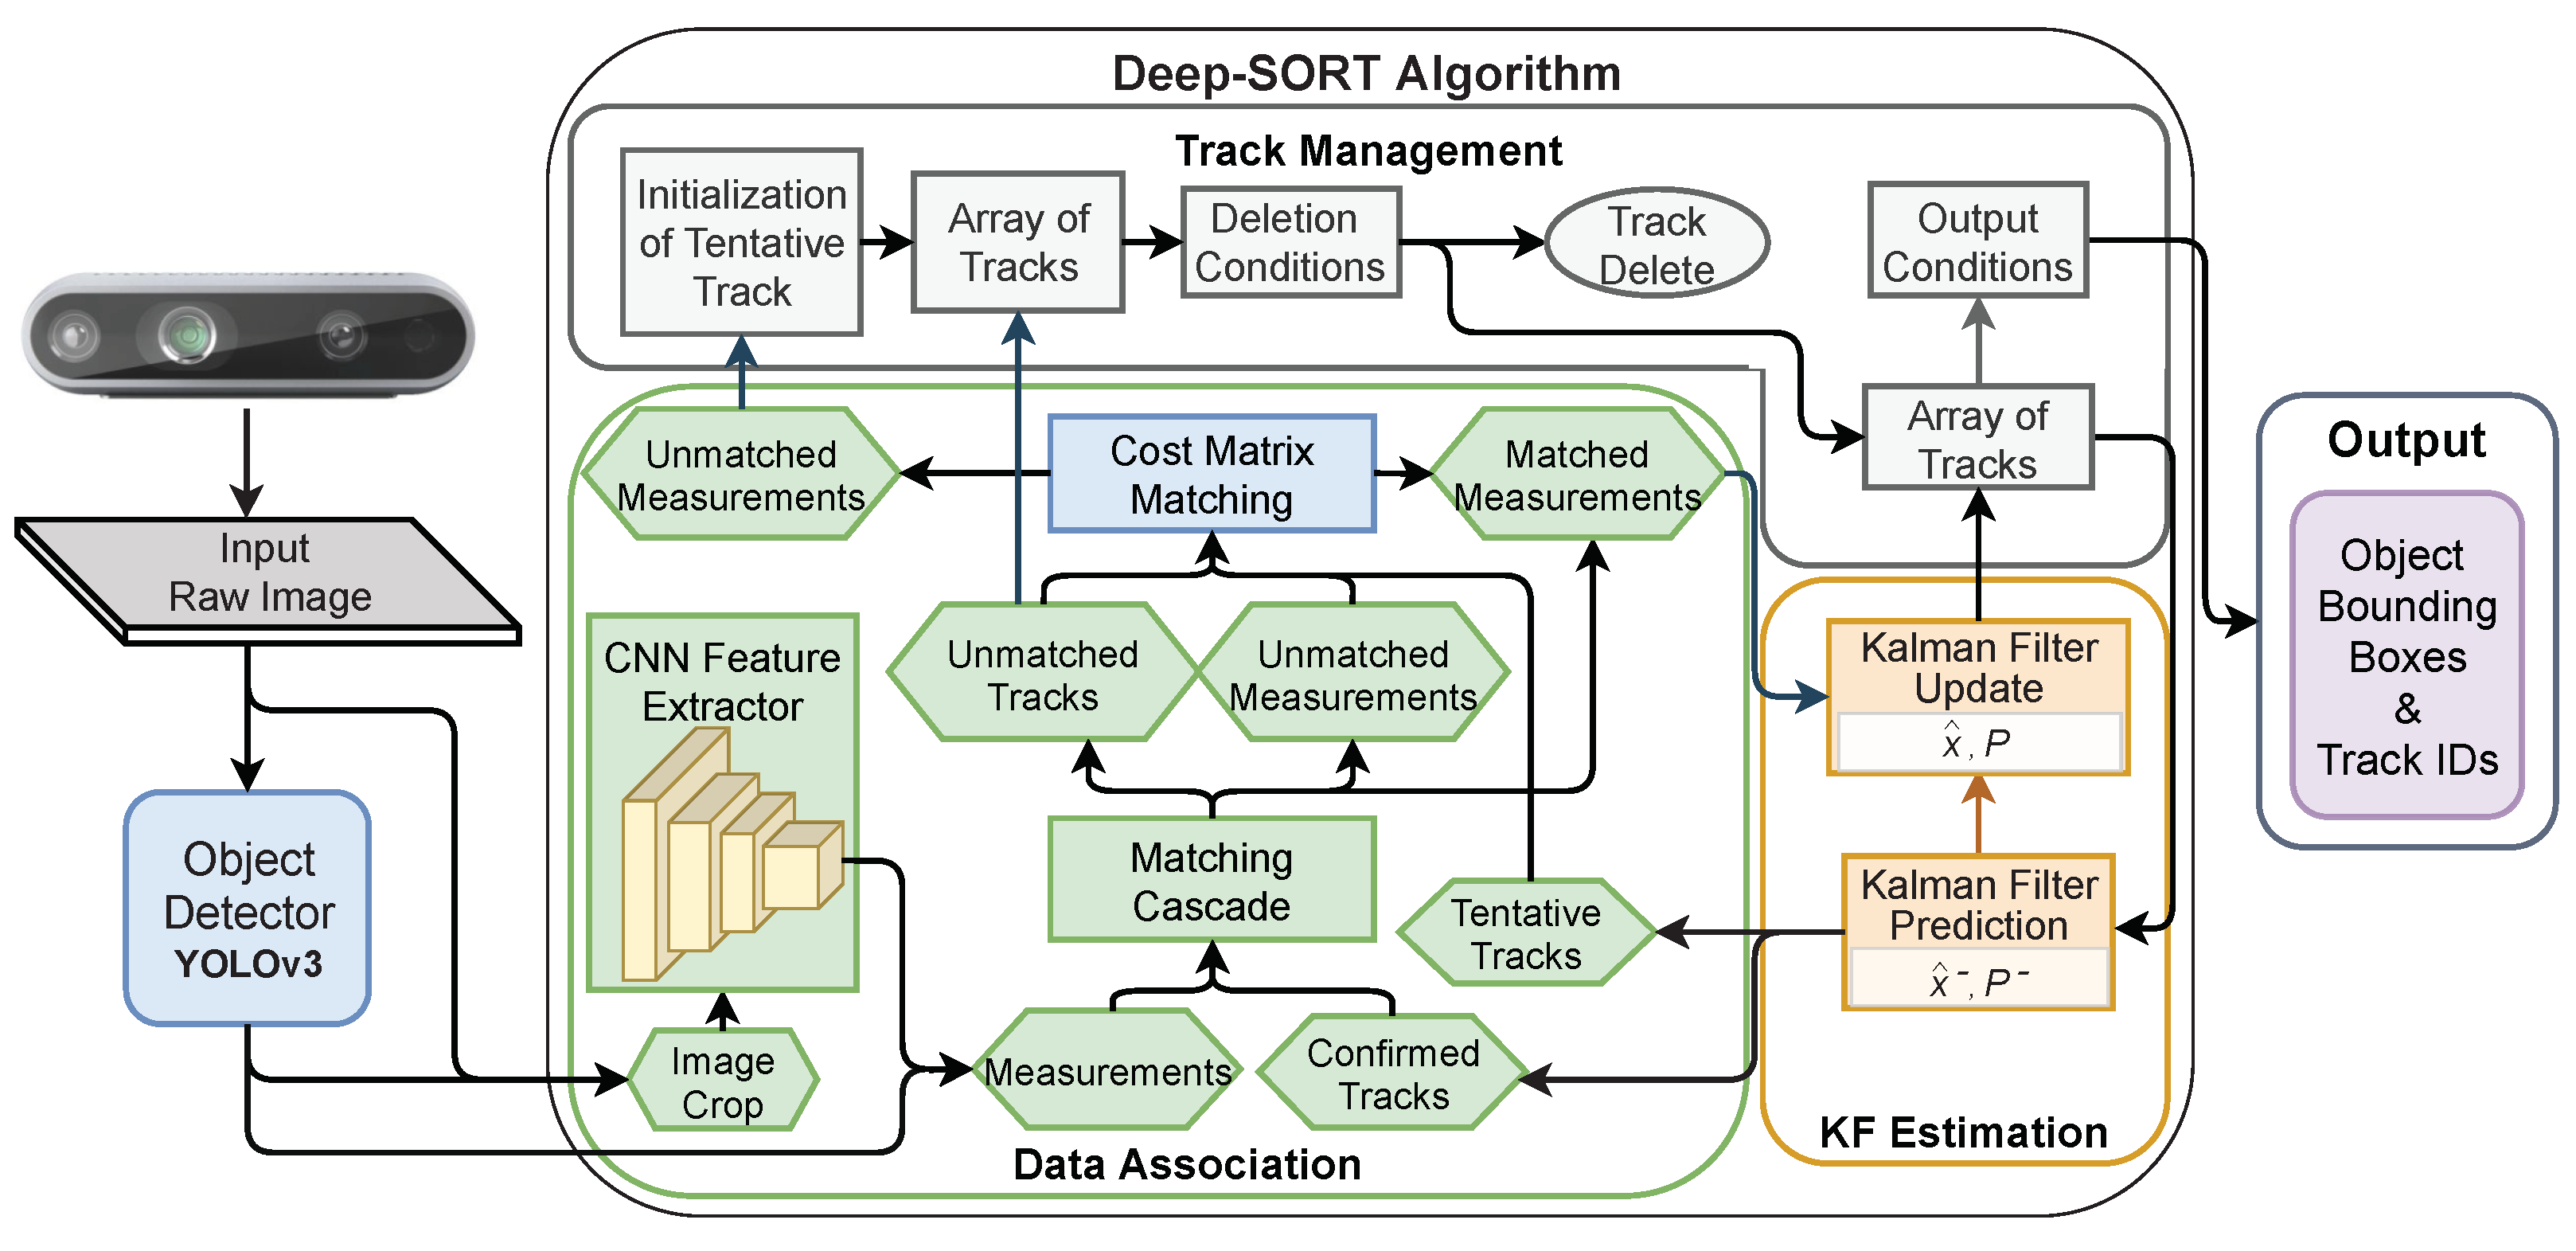
\includegraphics[width=0.9\textwidth]{Imagenes/Propias/DeepSort.png}
    \caption[Esquema general de DeepSORT]{
    Esquema general de DeepSORT. El método combina predicción mediante filtro de Kalman, asociación de detecciones y un descriptor de apariencia obtenido con una red convolucional, lo que ayuda a mantener identidades cuando el movimiento por sí solo no basta. Fuente: reproducido de \citep{PereiraDeepSORT2022}.
    }
    \label{fig:deepsort-esquema}
\end{figure}

Este enfoque puede reducir cambios de identidad en escenarios donde la apariencia visual ayuda a distinguir personas, como vigilancia o seguimiento de peatones. Sin embargo, en fútbol broadcast la apariencia puede ser menos discriminativa, ya que muchos jugadores del mismo equipo llevan equipaciones casi idénticas y las cajas pueden tener baja resolución. Además, entrenar o utilizar descriptores de reidentificación robustos para jugadores concretos requiere datos adicionales que no siempre están disponibles.

Otra alternativa relevante es OC-SORT, propuesto por \citet{CaoOCSORT2023}. Este método revisa el uso del filtro de Kalman en tracking y plantea una asociación más centrada en las observaciones reales, reduciendo errores acumulados durante oclusiones o movimientos no lineales. Este enfoque resulta interesante para deportes, ya que los jugadores no siempre siguen trayectorias suaves y pueden realizar cambios bruscos de dirección.

Frente a estas alternativas, ByteTrack resulta atractivo para sistemas de análisis deportivo por su equilibrio entre simplicidad, eficiencia y robustez ante detecciones de baja confianza. Su enfoque permite recuperar objetos que un tracker convencional podría descartar prematuramente, algo especialmente útil en escenas con oclusiones, agrupaciones de jugadores o detecciones inestables.